\documentclass[aspectratio=169]{beamer}
\usetheme[progressbar=foot,numbering=fraction]{metropolis} % Use metropolis theme

\usepackage{booktabs}
\usepackage{graphics, graphicx, svg}
\usepackage{amsmath}      % Math environments
\usepackage{amssymb}
\usepackage{url}
\usepackage{longtable}
\usepackage{tikz}
\usetikzlibrary{positioning}

\usepackage[backend=biber,
            style=authortitle,
            maxnames=2,
            isbn=false,
            sortcites=true,
            hyperref=false,
            url=false]{biblatex}
\addbibresource{mylit.bib}
\setbeamerfont{footnote}{size=\tiny}
\title{Application of FracMinHash to analyse the phylogenetic context of \textit{Phytophthora}}

\date{\today}
\author{ Felix Seidel \\
\href{mailto:felix.seidel@student.uni-tuebingen.de}{felix.seidel@student.uni-tuebingen.de}
}
\begin{document}

\maketitle

\begin{frame}{Overview}
    \tableofcontents
\end{frame}

\section{A short story}
\begin{frame}{The setting}
    \begin{figure}
        \centering
        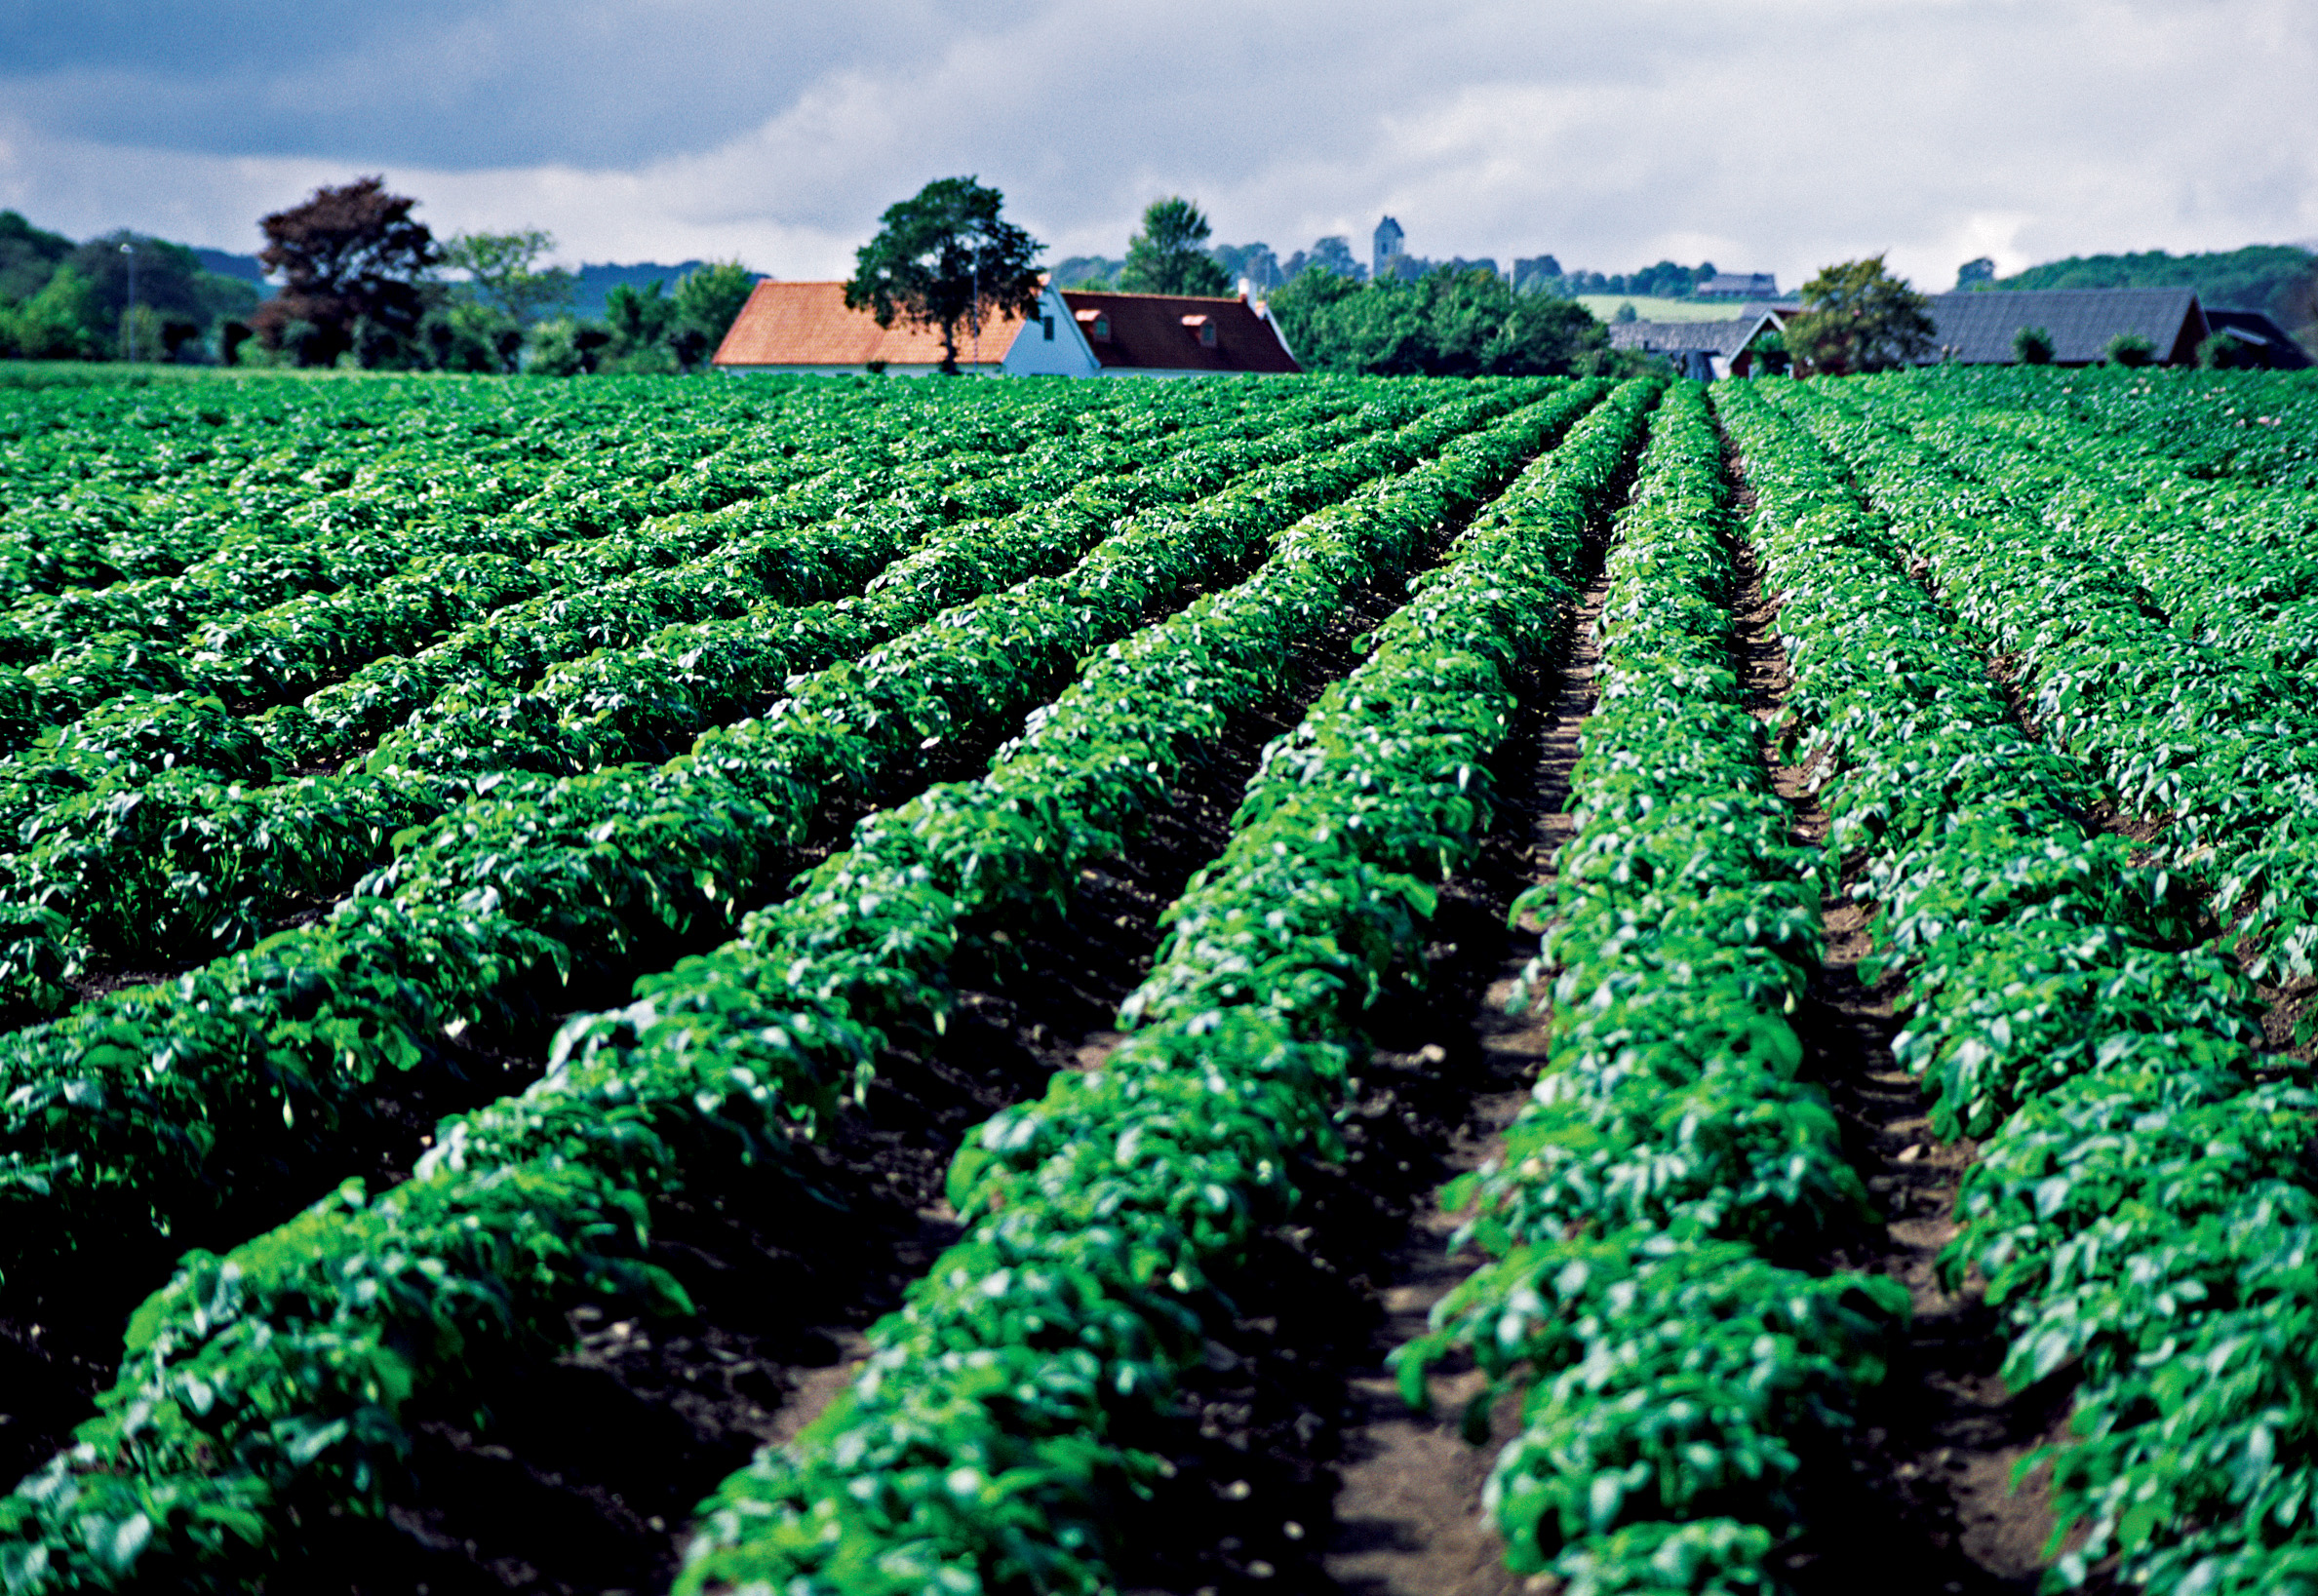
\includegraphics[width=0.5\textwidth]{figures/potato_farm.jpg}
        \caption{A potato farm in Sweden\footnote{Magnusson, \url{https://flic.kr/p/85qcc9}, CC BY-ND 2.0}.}
        \label{fig:farm}
    \end{figure}
\end{frame}

\begin{frame}{The trace}
\begin{columns}
    \begin{column}{0.5\textwidth}
        \begin{figure}
            \centering
            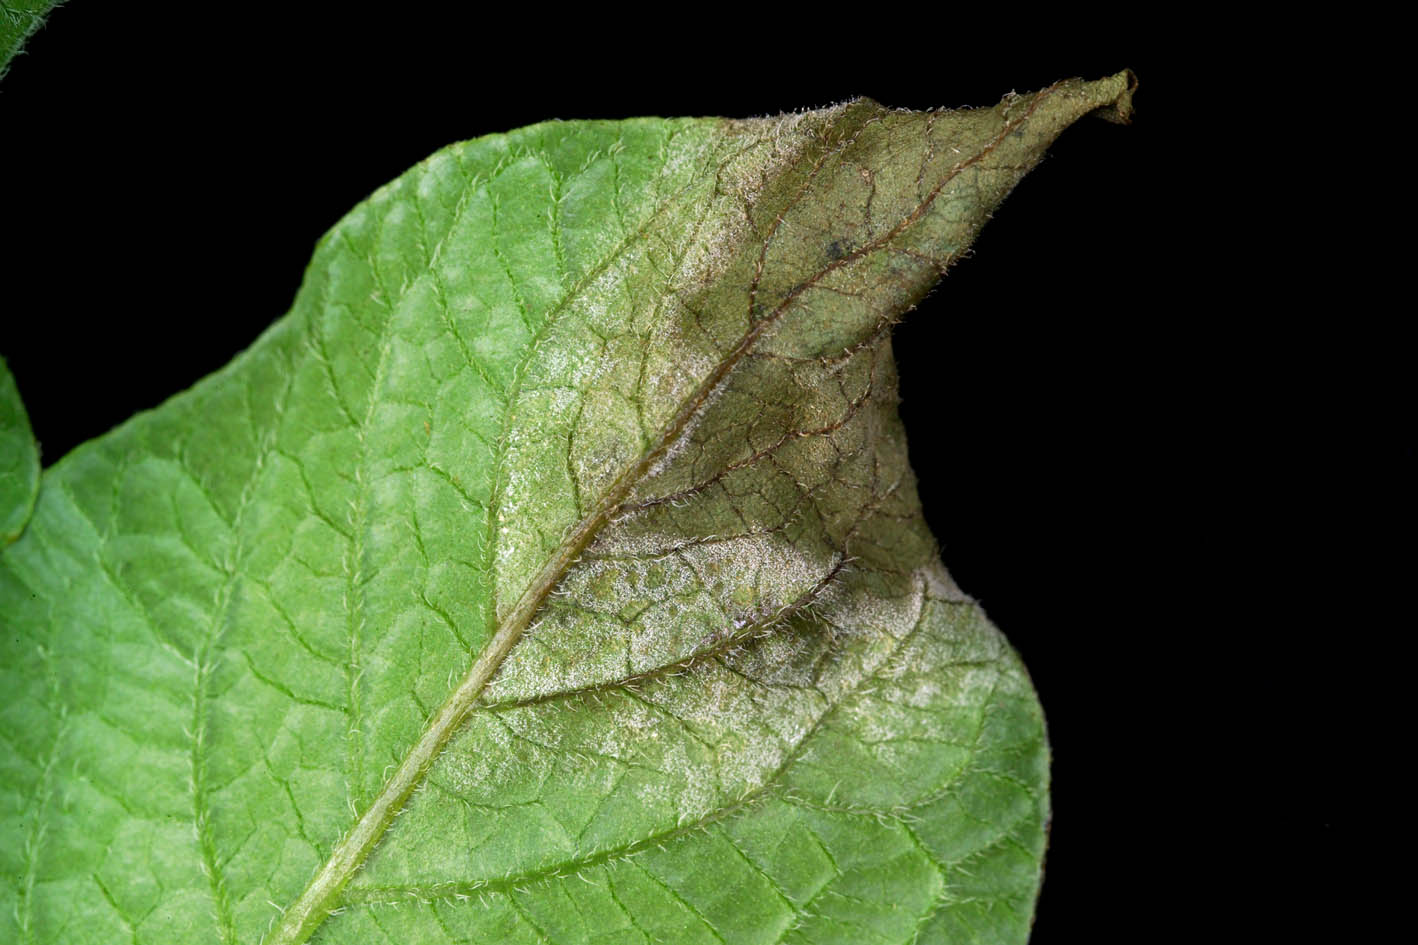
\includegraphics[width=1.0\textwidth]{figures/infestans_leaf.jpg}
            \caption{Infected potato plant\footnotemark{}.}
            \label{fig:infestans_leaf}
        \end{figure}
    \end{column}
    \begin{column}{0.5\textwidth}
        \begin{figure}
            \centering
            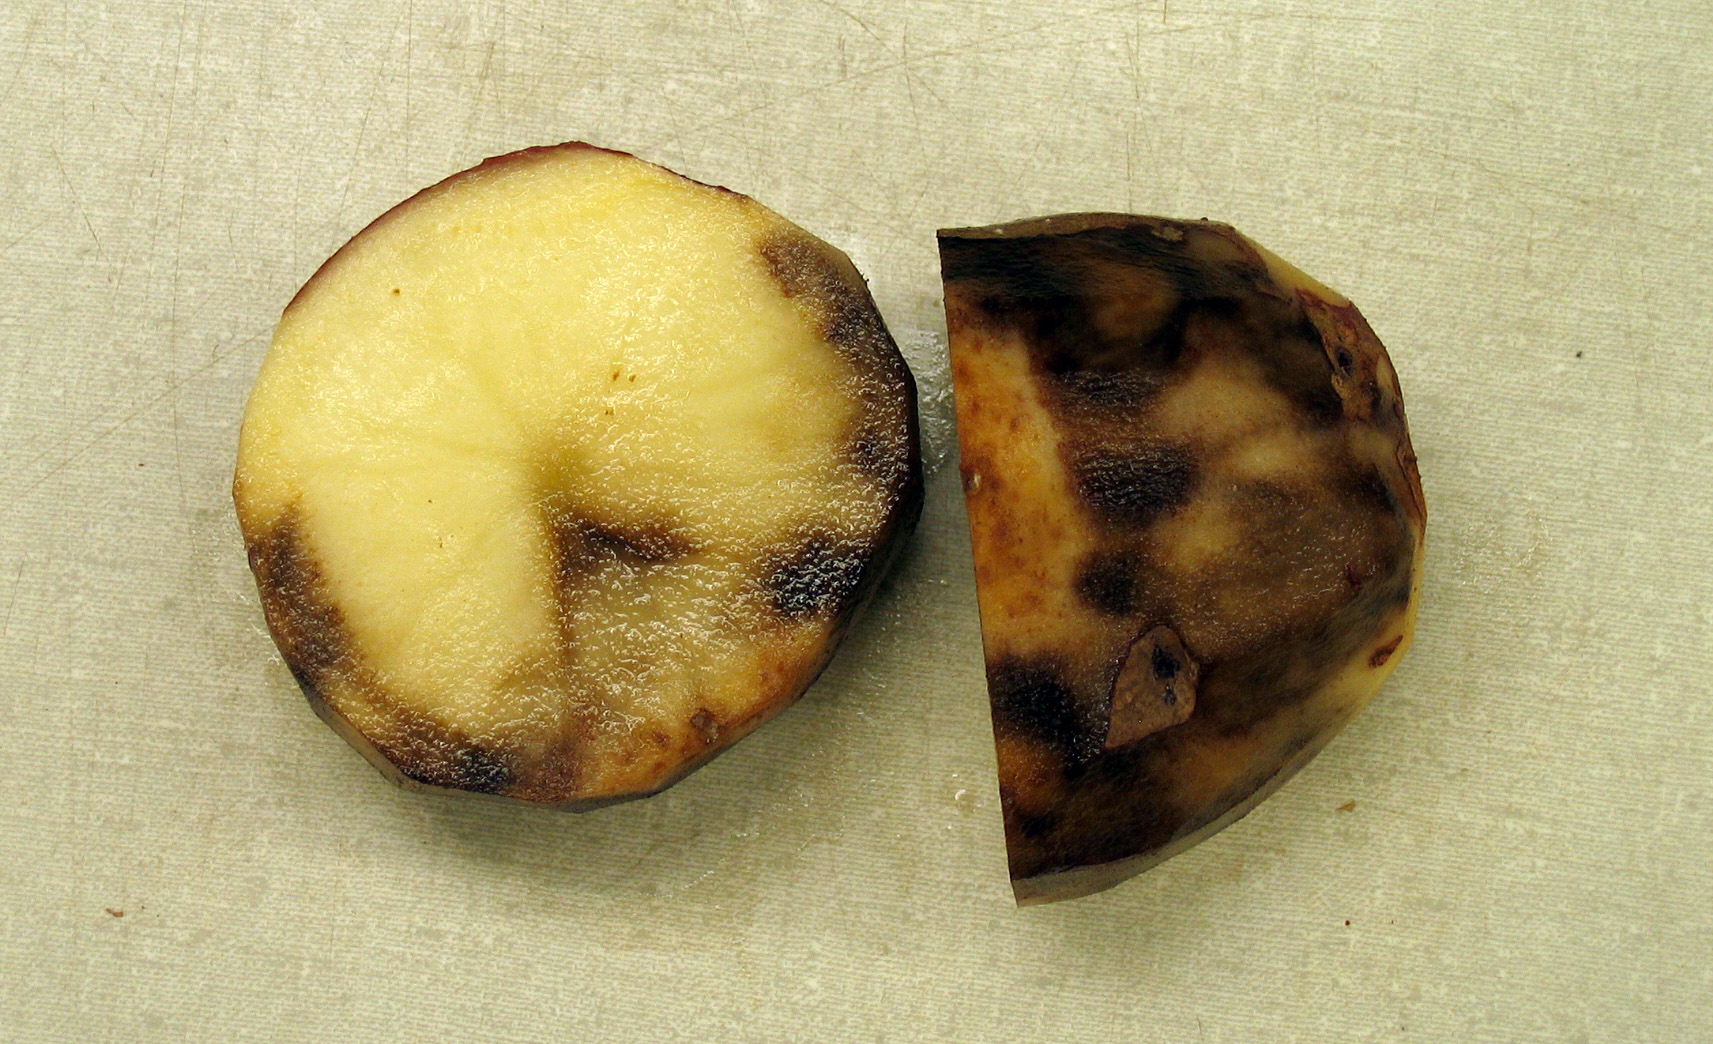
\includegraphics[width=1.0\textwidth]{figures/infestans_potato.jpg}
            \caption{Infected potato tuber\footnotemark{}.}
            \label{fig:infestans_tuber}
        \end{figure}
    \end{column}
\end{columns}
\footnotetext{Cooke, \url{https://flic.kr/p/nPy5Qa}, CC BY-SA 2.0}
\footnotetext{Millet, \url{https://flic.kr/p/qRXVt}, CC BY-NC-ND 2.0}
\end{frame}

\begin{frame}{The villain: \textit{Phytophthora}}
    \begin{columns}
        \begin{column}{0.3\textwidth}
            \centering
            \textit{Phytophthora\\infestans}
        \end{column}
        \begin{column}{0.3\textwidth}
            \centering
            \textit{Phytophthora\\cinnamomi}
        \end{column}
        \begin{column}{0.3\textwidth}
            \centering
            \textit{Phytophthora\\ramorum}
        \end{column}
    \end{columns}
\end{frame}

\begin{frame}{The hero?}
    \begin{columns}
        \begin{column}{0.3\textwidth}
            \centering
            \textbf{Research on Phylogeny}\footnotemark{}\footnotemark{}
        \end{column}
        \begin{column}{0.3\textwidth}
            \centering
            \textbf{Research on effector proteins\footnotemark{} and genome
            architecture\footnotemark{}}
        \end{column}
        \begin{column}{0.3\textwidth}
            \centering
            \textbf{Research on impact on microbial communities\footnotemark}
        \end{column}
    \end{columns}
    \footnotetext{\cite{yangExpandedPhylogenyGenus2017}}
    \footnotetext{\cite{abadPhytophthoraTaxonomicPhylogenetic2023a}}
    \footnotetext{\cite{raffaeleAnalysesGenomeArchitecture2010}}
    \footnotetext{\cite{dongTwospeedGenomesFilamentous2015}}
    \footnotetext{\cite{solis-garciaPhytophthoraRootRot2020}}
\end{frame}

\section{Background}
\begin{frame}{Phylogenetic Trees \footcite{scornavaccaSplitsUnrootedPhylogenetic2010}\footcite{bryantNeighborNetImprovedAlgorithms2023}\footcite{bagciMicrobialPhylogeneticContext2021}}
    \begin{columns}
        \begin{column}{0.5\textwidth}
            \begin{itemize}
                \item $X$: set of $n$ taxa
                \item $D$: distance matrix for $X$
                \item $S = A | B$: a bipartition of $X$ (split) based on $D$
                \item $\omega(S)$: the weight of $S$
                \item $\Sigma$: the set of all splits
            \end{itemize}
        \end{column}
        \begin{column}{0.5\textwidth}
            \begin{figure}
                \tikzstyle{main} = [draw, circle, fill] \tikzstyle{color_edge} =
                [color=mLightGreen]
                \begin{tikzpicture}[node distance={10mm}, minimum size={2mm},
                    inner sep={0pt}, thick] 
                    
                    \node[](l0){}; 
                    \node[below = of l0](l1){}; 
                    \node[below = of l1](l2){}; \node[below = of l2](l3){};
              
                    \node[main, right = 5mm of l1](abc){};
                    \node[main, right = 5mm of l2] (ba){} edge[color_edge](abc);
                    \node[right = 0mm of l3] (b) {B} edge(ba);
                    \node[right = 10mm of l3](a) {A} edge(ba);
                    \node[right = 0mm of l0] (c) {C} edge(abc);
                    \node[right = 10mm of l0] (d) {D} edge (abc);
                \end{tikzpicture}
            \end{figure}
        \end{column}
    \end{columns} 
\end{frame}

\begin{frame}{Phylogenetic Outlines \footcite{scornavaccaSplitsUnrootedPhylogenetic2010}\footcite{bryantNeighborNetImprovedAlgorithms2023}\footcite{bagciMicrobialPhylogeneticContext2021}}
    \begin{columns}
        \begin{column}{0.5\textwidth}
            \begin{itemize}
                \item $X$: set of $n$ taxa
                \item $D$: distance matrix for $X$
                \item $S = A | B$: a bipartition of $X$ (split) based on $D$
                \item $\omega(S)$: the weight of $S$
                \item $\Sigma$: the set of all splits
            \end{itemize}
        \end{column}
        \begin{column}{0.5\textwidth}
            \begin{figure}
                \tikzstyle{main} = [draw, circle, fill]
                \tikzstyle{color_edge} = [color=mLightGreen]
                \begin{tikzpicture}[node distance={10mm}, minimum size={2mm},
                    inner sep={0pt}, thick] 
                    
                    \node[](l0){};
                    \node[below = of l0](l1){};
                    \node[below = of l1](l2){};
                    \node[below = of l2](l3){};
                    \node[below = of l3](l4){};

                    \node[right = 20mm of l0](c){C};
                    \node[main, right = 20mm of l1](i1){} edge(c);
                    \node[main, right = 10mm of l2](i2){} edge[color_edge](i1);
                    \node[main, right = 30mm of l2](i4){} edge(i1);
                    \node[main, right = 20mm of l3](i3){} edge(i2) edge[color_edge](i4);

                    \node[right = 0mm of l2](b) {B} edge(i2);
                    \node[right = 20mm of l4](a) {A} edge(i3);
                    \node[right = 40mm of l2](d) {D} edge(i4);
                \end{tikzpicture}
            \end{figure}
        \end{column}
    \end{columns} 
\end{frame}

\begin{frame}{Phylogenetic Context \footcite{bagciMicrobialPhylogeneticContext2021}}
    \begin{figure}
        \tikzstyle{main} = [draw, circle, fill]
        \tikzstyle{draft} = [text=mLightGreen]
        \tikzstyle{color_edge} = [color=mLightGreen]
        \begin{tikzpicture}[node distance={10mm}, minimum size={2mm},
            inner sep={0pt}, thick] 
            
            \node[](l0){};
            \node[below = of l0](l1){};
            \node[below = of l1](l2){};
            \node[below = 5mm of l1](l15){};
            \node[below = of l2](l3){};
            \node[below = 5mm of l2](l25){};
            \node[below = of l3](l4){};

            \node[right = 20mm of l0](c){C};
            \node[main, right = 20mm of l1](i1){} edge(c);
            \node[main, right = 18mm of l15](i10){} edge(i1);
            \node[main, right = 10mm of l2](i2){} edge(i10);
            \node[main, right = 30mm of l2](i4){} edge(i1);
            \node[main, right = 28mm of l25](i20){} edge(i4);
            \node[main, right = 20mm of l3](i3){} edge(i2) edge(i20);
            

            \node[right = 0mm of l2](b) {B} edge(i2);
            \node[right = 20mm of l4](a) {A} edge(i3);
            \node[right = 40mm of l2](d) {D} edge(i4);
            \node[draft, below right = 5mm and 35mm of l3](unkown){?} edge[color_edge](i20);
        \end{tikzpicture}
    \end{figure}
\end{frame}

\begin{frame}{FracMinHash \footcite{irberLightweightCompositionalAnalysis2022} (1)}
    Idea: Hash $k$-mers and keep values smaller or equal to a threshold
    \begin{itemize}[<+->]
        \item Sequence: $ATGCATGATG$
        \item $k$-mers: $ATG, TGC, GCA, CAT, ATG, TGA, GAT, ATG$
        \item hash values: $1, 8, 3, 4, 1, 10, 6, 1$
        \item define threshold: $3$
        \item FracMinHash sketch: $\{1, 3\}$
    \end{itemize}
\end{frame}

\begin{frame}{FracMinHash \footcite{irberLightweightCompositionalAnalysis2022} (2)}
    \begin{itemize}
        \item $W$: input sequence
        \item $h$: hash function producing values in $[0, H]$
        \item $s$: scaling parameter $0 < s \leq H$
        \item $k(W)$: set of $k$-mers of $W$
    \end{itemize}
    \begin{align}
        \mathbf{FRAC}_s(W) = \{h(w) \leq \frac{H}{s} ~|~ \forall w \in k(W)\}
    \end{align}
\end{frame}

\begin{frame}{From sketches to distances \footcite{heraDerivingConfidenceIntervals2023}}
    \begin{align}
        J_{frac}(A, B) = \frac{1}{1 - (1 - \frac{1}{s})^{|A \cup B|}} \frac{|\mathbf{FRAC}_s(A) \cap \mathbf{FRAC}_s(B)|}{|\mathbf{FRAC}_s(A) \cup \mathbf{FRAC}_s(B)|}
    \end{align}
    \begin{align}
        D_{frac}(A, B) = 1 - (\frac{2 J_{frac}(A, B)}{1+J_{frac}(A, B)})^{\frac{1}{k}}
    \end{align}
\end{frame}


\section{Phylogenetic Context of \textit{Phytophthora}}
\begin{frame}{The implementation with \texttt{fmhdist} (1)}
    \begin{columns}
        \begin{column}{0.5\textwidth}
            \tikzstyle{main} = [rectangle, rounded corners, minimum width=4cm, minimum height=1cm,text centered, draw]
            \tikzstyle{focus} = [rectangle, rounded corners, minimum width=4cm, minimum height=1cm,text centered, draw=mDarkTeal, fill=mDarkTeal, text=black!2]
            \tikzstyle{arrow} = [thick,->,>=stealth]
            \begin{tikzpicture}[node distance=1.5cm]
                \node (db)[focus]{\texttt{fmhdist db}};
                \node (sketch)[main, below of = db]{\texttt{fmhdist sketch}};
                \node (refdist)[main, below of = sketch]{\texttt{fmhdist ref\_dist}};
                \node (outline)[main, below of = refdist]{\texttt{fmhdist outline}};

                \draw [arrow] (db) -- (sketch);
                \draw [arrow] (sketch) -- (refdist);
                \draw [arrow] (refdist) -- (outline);
            \end{tikzpicture}
        \end{column}
        \begin{column}{0.5\textwidth}
            \begin{itemize}
                \item Input: List of NCBI accession codes
                \item Sketching parameters: $s$, $k$, $h$ and random seed for $h$
                \item Output: Reference database
            \end{itemize}
        \end{column}
        \end{columns}   
\end{frame}

\begin{frame}{The implementation with \texttt{fmhdist} (2)}
    \begin{columns}
        \begin{column}{0.5\textwidth}
            \tikzstyle{main} = [rectangle, rounded corners, minimum width=4cm, minimum height=1cm,text centered, draw]
            \tikzstyle{focus} = [rectangle, rounded corners, minimum width=4cm, minimum height=1cm,text centered, draw=mDarkTeal, fill=mDarkTeal, text=black!2]
            \tikzstyle{arrow} = [thick,->,>=stealth]
            \begin{tikzpicture}[node distance=1.5cm]
                \node (db)[main]{\texttt{fmhdist db}};
                \node (sketch)[focus, below of = db]{\texttt{fmhdist sketch}};
                \node (refdist)[main, below of = sketch]{\texttt{fmhdist ref\_dist}};
                \node (outline)[main, below of = refdist]{\texttt{fmhdist outline}};

                \draw [arrow] (db) -- (sketch);
                \draw [arrow] (sketch) -- (refdist);
                \draw [arrow] (refdist) -- (outline);
            \end{tikzpicture}
        \end{column}
        \begin{column}{0.5\textwidth}
            \begin{itemize}
                \item Input: List of paths to FASTA files
                \item Sketching parameters: $s$, $k$, $h$ and random seed for $h$
                \item Output: sketches and their coordinates
            \end{itemize}
        \end{column}
        \end{columns}   
\end{frame}

\begin{frame}{The implementation with \texttt{fmhdist} (3)}
    \begin{columns}
        \begin{column}{0.5\textwidth}
            \tikzstyle{main} = [rectangle, rounded corners, minimum width=4cm, minimum height=1cm,text centered, draw]
            \tikzstyle{focus} = [rectangle, rounded corners, minimum width=4cm, minimum height=1cm,text centered, draw=mDarkTeal, fill=mDarkTeal, text=black!2]
            \tikzstyle{arrow} = [thick,->,>=stealth]
            \begin{tikzpicture}[node distance=1.5cm]
                \node (db)[main]{\texttt{fmhdist db}};
                \node (sketch)[main, below of = db]{\texttt{fmhdist sketch}};
                \node (refdist)[focus, below of = sketch]{\texttt{fmhdist ref\_dist}};
                \node (outline)[main, below of = refdist]{\texttt{fmhdist outline}};

                \draw [arrow] (db) -- (sketch);
                \draw [arrow] (sketch) -- (refdist);
                \draw [arrow] (refdist) -- (outline);
            \end{tikzpicture}
        \end{column}
        \begin{column}{0.5\textwidth}
            \begin{itemize}
                \item Input: reference databse (\texttt{fmhdist db} or \texttt{fmhdist sketch}), query sketches (\texttt{fmhdist sketch})
                \item Distance threshold
                \item Output: distance matrix
            \end{itemize}
        \end{column}
        \end{columns}   
\end{frame}

\begin{frame}{The implementation with \texttt{fmhdist} (4)}
    \begin{columns}
        \begin{column}{0.5\textwidth}
            \tikzstyle{main} = [rectangle, rounded corners, minimum width=4cm, minimum height=1cm,text centered, draw]
            \tikzstyle{focus} = [rectangle, rounded corners, minimum width=4cm, minimum height=1cm,text centered, draw=mDarkTeal, fill=mDarkTeal, text=black!2]
            \tikzstyle{arrow} = [thick,->,>=stealth]
            \begin{tikzpicture}[node distance=1.5cm]
                \node (db)[main]{\texttt{fmhdist db}};
                \node (sketch)[main, below of = db]{\texttt{fmhdist sketch}};
                \node (refdist)[main, below of = sketch]{\texttt{fmhdist ref\_dist}};
                \node (outline)[focus, below of = refdist]{\texttt{fmhdist outline}};

                \draw [arrow] (db) -- (sketch);
                \draw [arrow] (sketch) -- (refdist);
                \draw [arrow] (refdist) -- (outline);
            \end{tikzpicture}
        \end{column}
        \begin{column}{0.5\textwidth}
            \begin{itemize}
                \item Input: distance matrix
                \item Image parameters (width, height, scaling, offset)
                \item Output: phylogenetic outline as SVG
            \end{itemize}
        \end{column}
        \end{columns}   
\end{frame}

\begin{frame}{An outline produced by \texttt{fmhdist}} 
    \begin{figure}
        \fontsize{7}{10}\selectfont
        \includesvg[width=0.85\textwidth]{figures/outline.svg}
        \caption{Outline based on FracMinHash distances of \textit{Phytophthora}
        reference sequences and fungal and bacterial query sequences (bold).
        Only some labels shown.}
        \label{fig:outlineMash}
    \end{figure}
\end{frame}

\begin{frame}{Compare this to Mash}
    \begin{figure}
        \fontsize{7}{10}\selectfont
        \includesvg[width=0.95\textwidth]{figures/outline_mash.svg}
        \caption{Outline based on Mash distances of \textit{Phytophthora}
        reference sequences and fungal and bacterial query sequences (bold).
        Only some labels shown.}
        \label{fig:outline}
    \end{figure}
\end{frame}

\begin{frame}{Origin of the hashes in the sketch of \textit{Phytophthora sojae}}
    \begin{figure}
        \fontsize{8}{10}\selectfont
        \centering
        \includesvg[width=0.7\textwidth]{figures/p_sojae_without_comp.svg}
        \caption{Hash counts in windows of the NW\_009258123.1 sequence of the \textit{Phytophthora sojae} reference genome.}
        \label{fig:counts_psoj}
    \end{figure}
\end{frame}

\begin{frame}{\dots and the corresponding sequence complexity\footcite{pirogovHighcomplexityRegionsMammalian2019}}
    \begin{figure}
        \fontsize{8}{10}\selectfont
        \centering
        \includesvg[width=0.7\textwidth]{figures/p_sojae_with_comp.svg}
        \caption{Hash counts and sequence complexity in windows of the
        NW\_009258123.1 sequence of the \textit{Phytophthora sojae} reference
        genome.}
        \label{fig:counts_psoj_comp}
    \end{figure}
\end{frame}

\begin{frame}{How about other genomes?}
    \begin{figure}
        \fontsize{8}{10}\selectfont
        \centering
        \includesvg[width=0.7\textwidth]{figures/p_infestans_with_comp.svg}
        \caption{Hash counts and sequence complexity in windows of the
        NW\_003303751.1 sequence of the \textit{Phytophthora infestans}
        reference genome.}
        \label{fig:counts_pinf_comp}
    \end{figure}
\end{frame}

\begin{frame}{Statistical analysis}
    \begin{table}
        \begin{tabular}{@{}lrrrr@{}}
        \toprule
        \textbf{}                           & $\textbf{$n$}$ & \textbf{$u$} & \textbf{$r$} &  \textbf{$p$}  \\ \midrule
        \textit{P. cambivora}               & 727        & 0          & -0.0272      &               \\
        \textit{P. betacei}                 & 26688      & 437        & 0.2446       & 4.5575e-265  \\
        \textit{P. cinnamomi}               & 10799      & 28         & -0.0933      & 4.3767e-19  \\
        \textit{P. infestans}               & 11173      & 37         & 0.1830       & 2.8352e-24   \\
        \textit{P. sojae}                   & 7339       & 74         & 0.1570       & 6.5134e-48    \\
        \textit{P. nicotianae}              & 2529       & 0          & -0.0042      &                         \\ \bottomrule
        \end{tabular}
        \caption{Excerpt of the statistical analysis of window ($w=10000$) hash
        counts and sequence complexity of \textit{Phytophthora} genomes.}
        \label{ta:hashCountComplexity}
      \end{table}
\end{frame}

\begin{frame}{Benchmarks}
    \begin{table}[]
        \centering
        \begin{tabular}{@{}lrrrrr@{}}
        \toprule
                        & \texttt{mash}\footcite{ondovMashFastGenome2016} (1)     & \texttt{mash} (6) & \texttt{sourmash}\footcite{irberLightweightCompositionalAnalysis2022} (1) & \texttt{fmhdist} (1) & \texttt{fmhdist} (6) \\ \midrule
        min (s) & 135                     &  44                     &  171              &  201                      & 75                         \\
        max (s) & 140                     &  58                     &  178              &  215                      & 91                         \\
        avg (s) & 137                     &  51                     &  174              &  208                      & 84                         \\ \bottomrule
        \end{tabular}
        \caption{Runtime comparison of three tools calculating sketches for
        sequences totalling $5.477$Gb. The number of threads is in parantheses.}
        \label{ta:performance}
      \end{table}
\end{frame}

\section{Conclusion}
\begin{frame}{Conclusion}
    \begin{columns}
        \begin{column}{0.5\textwidth}
            \textbf{Summary}
            \begin{itemize}
                \item FracMinHash is a solid foundation for Phylogenetic outlines.
                \item Distantly related genomes are better represented.
                \item Some \textit{Phytophthora} genomes have windows with
                unusual densities.
            \end{itemize}
        \end{column}
        \begin{column}{0.5\textwidth}
            \textbf{Open questions}
            \begin{itemize}
                \item What happens to the left and the right of windows with
                unusual densities?
                \item Can we use this method to assign a label to a draft genome?
            \end{itemize}
        \end{column}
    \end{columns}
\end{frame}

\begin{frame}[standout]
    Thanks!
\end{frame}
\end{document}